\documentclass[12pt,a4paper,oneside,titlepage]{article}
\usepackage[authoryear,longnamesfirst,round, comma]{natbib}               %Zitieren
\usepackage{graphicx}             %Graphik-Paket
\usepackage{color}
\usepackage[USenglish]{babel}     %Spracheinstellung USEnglish
\usepackage[utf8]{inputenc}       %Umlaute & Akzente
\usepackage{lmodern}              %Computer-Modern als Vektorgrafiken

\usepackage{setspace}             %Zeilenabstand 1,5
\onehalfspacing
%Zeilenabstand vor und nach Gleichungen ändern
\makeatletter
\g@addto@macro\normalsize{%
  \setlength\abovedisplayskip{2pt}
  \setlength\belowdisplayskip{5pt}
  \setlength\abovedisplayshortskip{0pt}
  \setlength\belowdisplayshortskip{0pt}
}
\makeatother

\usepackage{geometry}             %Seitenränder anpassen
\geometry{a4paper,left=30mm,right=25mm, top=2cm, bottom=3cm}



\usepackage{microtype}            %besseres Schriftbild
\usepackage{footmisc}             %Fußnoten

\usepackage[tbtags]{mathtools}            %Mathematische Symbole
\usepackage{amsmath, amsthm, amssymb, amsfonts}    %bessere mathematische Formeln

\usepackage{booktabs}             %bessere Tabellen
\usepackage{marvosym}             %Symbole einfügen


\usepackage{titletoc}			  %Inhaltsverzeichnis anpassen
\dottedcontents{section}[3em]{\bfseries}{2.9em}{1pc}
\dottedcontents{subsection}[4em]{}{3.3em}{1pc}

\usepackage[small]{titlesec}     %Überschriften anpassen

\usepackage{epstopdf}            %include Matlab Figures


\renewcommand{\thesection}{\Roman{section}}  %Römische Zahlen bei Überschrift
\renewcommand{\thesubsection}{\thesection.\Roman{subsection}}





\begin{document}
\parindent 0pt %kein Erstzeileneinzug
\begin{titlepage}
	\centering
	
\includegraphics[width=0.8\textwidth]{pictures/LogoFU}\par\vspace{1cm}
	{\scshape\large Freie Universität Berlin \par}
	\vspace{1cm}
	{\scshape\large Seminar Paper in "Recent Research in Macroeconomics"\par}
	\vspace{1.5cm}
	{\LARGE\bfseries Replication of Erceg \& Lindé (2012):\par}
	\vspace{0.5cm}
	{\Large\bfseries Is there a Fiscal Free Lunch in a Liquidity Trap?\par}
	\vspace{2cm}
	{\Large\itshape Denis Maciel \& Tobias Müller\par}
	\vfill
	supervised by\par
	Prof. Dr. Mathias \textsc{Trabandt}

	\vfill

% Bottom of the page
	{\large \today\par}
\end{titlepage}


\doublespacing
\tableofcontents

\pagebreak[4]
\listoffigures
\listoftables
\newpage

\section{Introduction}

The financial crisis in 2008 and the following worldwide recession marked a turning point in the economic and public debate about optimal fiscal and monetary policy. In the aftermath of the great recession, economists discussed about the effects of an expansionary fiscal policy to stabilize the economy and stimulate the private sector. The focus of the analysis has been on the size of the fiscal multiplier and the rise of output in response to a government spending hike.
\par
\bigskip
The economic crisis challenged the state of the art of the economic research at this time. To prevent the economy from falling in a prolonged recession, governments and central banks launched unconventional and in part uncharted measures. When central banks reduced the interest rates down to the zero lower bound, fiscal policy became more important to counteract the deflationary spiral and the large output gap of the recession. The increasing literature about fiscal policy and the government spending multiplier, as well as new developments in general equilibrium models, suggest the effectiveness of government spending, when the nominal interest rate hits the zero lower bound. Normally, the fiscal multiplier is not only larger in an environment of a liquidity trap, but also comes together with minimal budgetary costs.
\par
\bigskip
Therefore, the authors Christopher Erceg and Jesper Lindé address in the paper \textit{"Is there a Fiscal Free Lunch in a liquidity trap?"} the question whether policymakers should limit the size of the government spending. As we see in this paper, the distinction between marginal and average size of the fiscal multiplier is crucial for policymakers to better understand the effects of the implemented policies. The paper also gives new insights into how fiscal spending and austerity measures impact the government budget in a liquidity trap. The authors contribute with their paper to the current discussion about the efficiency of fiscal policy when monetary policy reaches its limit. By replicating the paper in Matlab \& Dynare, we followed the aims of the seminar to develop economic intuition and quantitative
methodological expertise, as well as the understanding of the current macroeconomic policy debates.
\par
\bigskip

Our paper is organized as follows. In Section II, we discuss briefly the current literature about the government spending multiplier and explain the main results of the analyzed paper. In Section III, we concentrate on the key equations of the paper, explain the structure of the model and explain the underlying microeconomics intuition of the simple New Keynesian model. In Section IV, we present the results of the impulse response to show how the model reacts to an exogenous consumption taste shock and government-spending shock. Furthermore, we interpret the shock parameters for better understanding of the dimension. We also give some impressions on how the results vary if we change the slope of the Phillips curve or the parameters of the monetary rule. In Section V, we dive deeper into the concept of multiplier and explain the distinction between \textit{marginal} and \textit{average} multiplier. We show that the variation of the fiscal multiplier depends highly on the size of the government response and the average contract duration (the Calvo parameter). In Section VI, we analyze the impacts of the increase in government spending on the government budget and answer the question wether there is a fiscal free lunch in a liquidity trap. In Section VII we provide some additional information on our workflow, which shall be useful for future participants of this seminar. We conclude our paper with the main takeaways and a short critique.


\section{Fiscal Policy and the Spending Multiplier }

Fiscal policy was often seen as inefficient and costly. In particular, the time-lag of the implementation of the fiscal spending and the crowing-out effect on the private sector were seen as some great obstacles to the use of public spending programs. Besides the theoretical economic arguments, there has been a quite considerable disagreement of model-based evidence on the effects of fiscal policy (see \citep{CoenenG..2010} and \citep{Coenen.2010}) All the analyses have in common that the outcome of fiscal spending depends on a series of different assumptions. The type, duration and funding of the fiscal stimulus are as important as the circumstances of the economic meltdown, the interaction with monetary policy and the scope for public finance. When we assume that a economic crisis normally has negative consequences for the current debt position of a country, as we could observe in affected countries by the euro crisis, the budgetary room for maneuver can be highly at risk in a situation when fiscal packages can normally be extraordinary effective. \citep{Afonso.2010}

New evidence on recent model-based economic research provided some new understanding whether fiscal policy can be an adequate response in a deep and prolonged recession when monetary policy reaches its limits. \citet{Eggertsson.2011}, \\citet{•} DAVID AND LEEPER 2011) and \citet{Christiano.2011} show that an increase in government spending can outsize the effect on output in a deep recession. Especially in prolonged liquidity traps, there can be a strong case for a fiscal stimulus on a temporary basis to jump start the economy and push it out of an economic downward spiral.
The key question of the paper "Is there a fiscal free lunch in a liquidity trap" concentrates on the magnitude of the government spending multiplier under different frameworks, the distinction between marginal and average effects and the impact of the fiscal policy on the government budget.


- NK framework

The impacts of higher spending or fiscal consolation measures in an environment of a liquidity trap when the nominal interest rate hits zero,

Fiscal policy can play a crucial role in stabilizing the economy during an economic crisis. Recent literature shows that the government spending multiplier is particularly large in recessions. Improvements in the economic research and new developments in New Keynesian Model literature after the financial crisis 2008 can help the political decision makers to better understand optimal policies in times of an great economic downturn. 

  - Fiscal spending in a liquidity trap is very efficient
  - Multiplier is high but decreases quickly...
  - results depend highly on the framework of the model - we show the level of price stickiness, monetary policy rule

\section{The Model}
In this section we describe and summarize the baseline illustration of the New Keynesian dynamic stochastic general equilibrium (DSGE) model \citet{Erceg.2014} use in their paper\footnote {Additional information and a more detailed derivation of the standard log-linearized version of the New Keynesian model can be found in the Online Appendix of the original paper.}. The New Keynesian DSGE model has a RBC-core, but allows two inefficiencies, so that shocks can cause deviations from the "natural level": monopolistic competition among firms and the Calvo model of firms' price setting. Therefore, the New Keynesian model addresses the deficits of the RBC-models and makes the more realistic assumptions that prices are not adjusted continuously and real world markets are not perfectly competitive. Consequently, monetary policy can affect the real interest rate, thus has real effects. The microfoundation allows a normative policy analysis.
\subsection*{Households}

The representative household decides the intertemporal consumption demand by maximizing
\begin{equation}
E_t \sum_{j=0}^\infty \beta^j \left\{ \frac{1}{1- \frac{1}{\sigma}} \left(C_{t+j} - C\nu_{t+j}\right)^{1-\frac{1}{\sigma}} - \frac{N_{t+j}^{1+\chi}}{1+\chi} + \mu_0F \left(\frac{MB_{t+j+1}(h)}{P_{t+j}}\right)\right\} \nonumber
\end{equation}
under the constraint\newline
$P_t(1+\tau_{C,t})C_t + B_{G,t} + MB_{t+1} = (1-\tau_{N,t})W_tN_t + (1+i_{t-1})B_{G,t-1} + MB-T_t + \Gamma_t,$
where 0 $< \beta > 1$ is the discount factor and $E_t$ the rational expectations operator. The utility function depends on the households current consumption $C_t$ as deviation from a “reference level” $C\nu_{t+j}$, where C is steady-state consumption, and a negative taste shock $\nu_t$ which reduces this reference level. The taste shock, we focus on in the next sections of the paper, therefore enters the model in the households utility function and affect the consumption decision of the household. The shock changes the marginal utility of consumption and so the willingness to consume the produced goods.\newline
The utility function also depends inversely on hours worked $N_t$. The inclusion of money, as a zero nominal interest asset, provides a rationale for the zero lower bound on nominal interest rates. By assuming that $\mu_0$ is arbitrarily small, changes in real money balances have negligible implications for seignorage in the model. The households budget constraint implies that the expenditure on goods and net purchases of government bonds $B_{G,t}$ equals the after-tax labor income $ \left(1 - \tau_{N,t} \right) W_tN_t$, minus a lump-sum tax $T_t$, plus a proportional share of the profits $\Gamma_t$ of all intermediate firms. The households optimal plan needs to satisfy the first order condition, so that we receive
\begin{align}
\vspace{-0.5cm} \left(C_t - C\nu_t\right)^{-\frac{1}{\sigma}}  - \lambda_tP_t \left(1 + \tau_{C,t} \right) = 0,\nonumber\\
-N_t^{\chi} + \lambda_t \left(1 - \tau_{N,t} \right) W_t = 0,\nonumber\\
-\lambda_t + \beta \left(1 + i_t \right) E_t\lambda_{t+1} = 0,\nonumber
\end{align}
and finally the Euler equation
\begin{equation}
\frac {\left(C_t - C\nu_t\right)^{-\frac{1}{\sigma}}}{\left(1 + \tau_{C,t} \right)} = \beta E_t \frac{\left(1 + i_t \right)}{1 + \pi_{t+1}} \frac{\left(C_{t+1} - C\nu_{t+1}\right)^{-\frac{1}{\sigma}}}{\left(1+ \tau_{C,t+1}\right)},
\end{equation}
and the aggregate labor supply relation
\begin{equation}
mrs_t \equiv \frac{N_t^\chi}{\left(C_t - C\nu_t\right)^{-\frac{1}{\sigma}}} = \frac{\left(1 - \tau_{N,t}\right)}{\left(1 + \tau_{C,t}\right)} \frac{W_t}{P_t}.
\end{equation}
The last equation shows that the marginal rate of substitution between consumption and labor must equal the real wage.
We have to mention that in our simple New Keynesian Model we set the sales tax $\tau_{C,t}$ equal to zero, to get the same results as in the paper.

\subsection*{Firms}
The production function of the firms is
\begin{equation}
Y_t = K^\alpha N_t^{1-\alpha},\vspace{-0.3cm} \nonumber
\end{equation}
where aggregate capital is fixed, but shares of the aggregate capital stock can be allocated across the firms. All firms choose the factor demand such that costs are minimized. The real factor costs per marginal product therefore are
\begin{equation}
\frac{MC_t}{P_t} = \frac{W_t/P_t}{\left(1 - \alpha \right) K^\alpha N_t^{-\alpha}}.
\end{equation}
The firm, which can reset its price in period t, chooses a price $\left(P_t^{opt} \right)$ and maximizes the problem
\begin{equation}
\max_{P_t^{opt}\left(f\right)} E_t \sum_{j=0}^\infty \xi_p^j \psi_{t,t+j} \left[ \left(1 + \pi \right)^j P_t^{opt}\left(f\right) - MC_{t+j} \right] Y_{t+j} \left(f\right),\nonumber
\end{equation}
where $\psi_{t,t+j}$ is the discount factor and $\xi$ the probability that the firm's price set in t will still be valid in period t+1. The demand function for the good $\left(f\right)$ which faces the firm is given by
\begin{equation}
Y_{t+j}\left(f\right) = \left[\frac{P_t \left(f\right)}{P_t} \right]^{\frac{-\left(1+\theta_p\right)}{\theta_p}} Y_t \nonumber,
\end{equation}
which varies with the relative price of the good, the substitution elasticity $\theta$ and the aggregate demand $Y_t$. The first order condition with optimal price $\left(P_t^{opt} \right)$ is
\begin{equation}
E_t \sum_{j=0}^\infty \xi_p^j \psi_{t,t+j} \left[ \frac{\left(1 + \pi \right)^j P_t^{opt}\left(f\right)}{1 + \theta_p} - MC_{t+j} \right] Y_{t+j}\left(f\right) = 0.
\end{equation}
For deriving the New Keynesian Phillips curve, we also need the average price of the final goods
\begin{equation}
P_t = \left[\left(1 - \xi_p\right)\left(P_t^{opt}\right)^{\frac{-1}{\theta_p}} + \xi_p \left(\left(1 + \pi\right)P_{t-1}\right)^{\frac{-1}{\theta_p}} \right]^{-\theta_p}.
\end{equation}
Finally, we have to derive the aggregate resource constraint
\begin{equation}
C_t + G_t \leq \left(\frac{P_t^*}{P_t}\right)^{\frac{\left(1+\theta_p\right)}{\theta_p}} K^\alpha N_t^{1-\alpha},
\end{equation}
where actual output $Y_t$ can be divided into private consumption and government spending $\left(Y_t \equiv C_t + G_t \right)$.\newline
By log-linearizing the equations (1) to (7) around the steady-state and some rearranging, we receive the key equations of the model used in the \citet{Erceg.2014} paper.

\subsection*{The Government}

The government budget constraint is given by
\begin{equation}
B_{G,t} = \left(1 + i_{t-1}\right)B_{G,t-1} + P_tG_t - \tau_{C,t}P_tC_t - \tau_{N,t}W_tN_t - T_t - MB_{t+1} + MB_t,  \nonumber
\end{equation}
where after scaling with $1/ P_tY_t$, the left side of the equation defines the end-of-period real government debt. In the model the government can issue bonds to finance the budget. As mentioned before, we set the consumption tax $\tau_{C,t}$ in our simplified model equal to zero for all t. The government charges the labor income with a constant tax rate $\tau_N$ according to the equation \[\tau_N = \frac{g_y}{s_N}\] with $g_y$ as the government share of steady-state output $\left(g_y = 0.2 \right)$ and the steady-state labor share $\left(s_N = 0.7\right)$.
The government also collects a lump-sum tax $\left(\tau_t \equiv T_t/P_tY)\right)$, which varies in time and is adjusted according to the evolution of the debt stock $\left(\tau_t = \varphi_b b_{G,t-1}\right)$. Therefore, the fiscal policy specifies that taxes respond to government debt, but does not affect other macro variables in the model. We set the tax rule parameter $\varphi_b$ equal to 0.01. Consequently, the evolution of the tax base depends mostly on the variation in labor tax revenues the first years after a negative taste shock. The government budget is zero in steady-state in the simple benchmark model.\newline
Monetary policy follows a Taylor rule which is subject to the zero lower bound.
\begin{equation}
i_t = max \left(-i, \gamma_{\pi} \pi_t + \gamma_x x_t\right)  \nonumber
\end{equation}
By setting the parameters $\gamma_{\pi}$ and $\gamma_x$ arbitrarily large, we assume that the monetary policy would completely stabilizes inflation and the output gap in absence of the the zero lower bound. In the next section, we also consider the alternative case where the parameters of the monetary policy rules are lower.\newline
Table \ref{tab:Tabel1} provides an overview over the parameter values, we use in our benchmark calculation.
\bigskip


\section{Impulse Response}

First, we focus on the impulse response of a large negative taste shock and a positive government spending shock in response to the fall in output. The main steps to reimplicate the New Keynesian model and the results of the \citet{Erceg.2014} paper are the following:
\begin{enumerate}
\item Write up the model equations in Dynare and set the parameter values provided in the paper\vspace{-0.3cm}
\item Solve the model without baseline shock, so that the nominal interest rate does not hit the zero lower bound and compute then impulse to government spending and consumption taste shock\vspace{-0.3cm}
\item Impose the ZLB on monetary policy and simulate effects of a large negative consumption demand shock, so that the economy hits the zero lower bound\vspace{-0.3cm}
\item Find the right parameter and shock values for an eight quarter liquidity trap in an environment of an positive government spending shock equal to one percentage point of steady-state output\vspace{-0.3cm}
\item Calculate the difference between the impulse responses of both shocks and the taste shock only to receive the effects of the government spending shock
\end{enumerate}
The large taste shock leads to a fall of the potential real interest rate $r^{pot}$. The length of the liquidity trap is defined on how long $r^{pot}$ remains below $-i$.
Figure \ref{IRnoinflation} gives the first impression of how the negative taste shock affects the key variables of the model: the real interest rate, the output gap, inflation and government debt to GDP.
\begin{figure}[p]
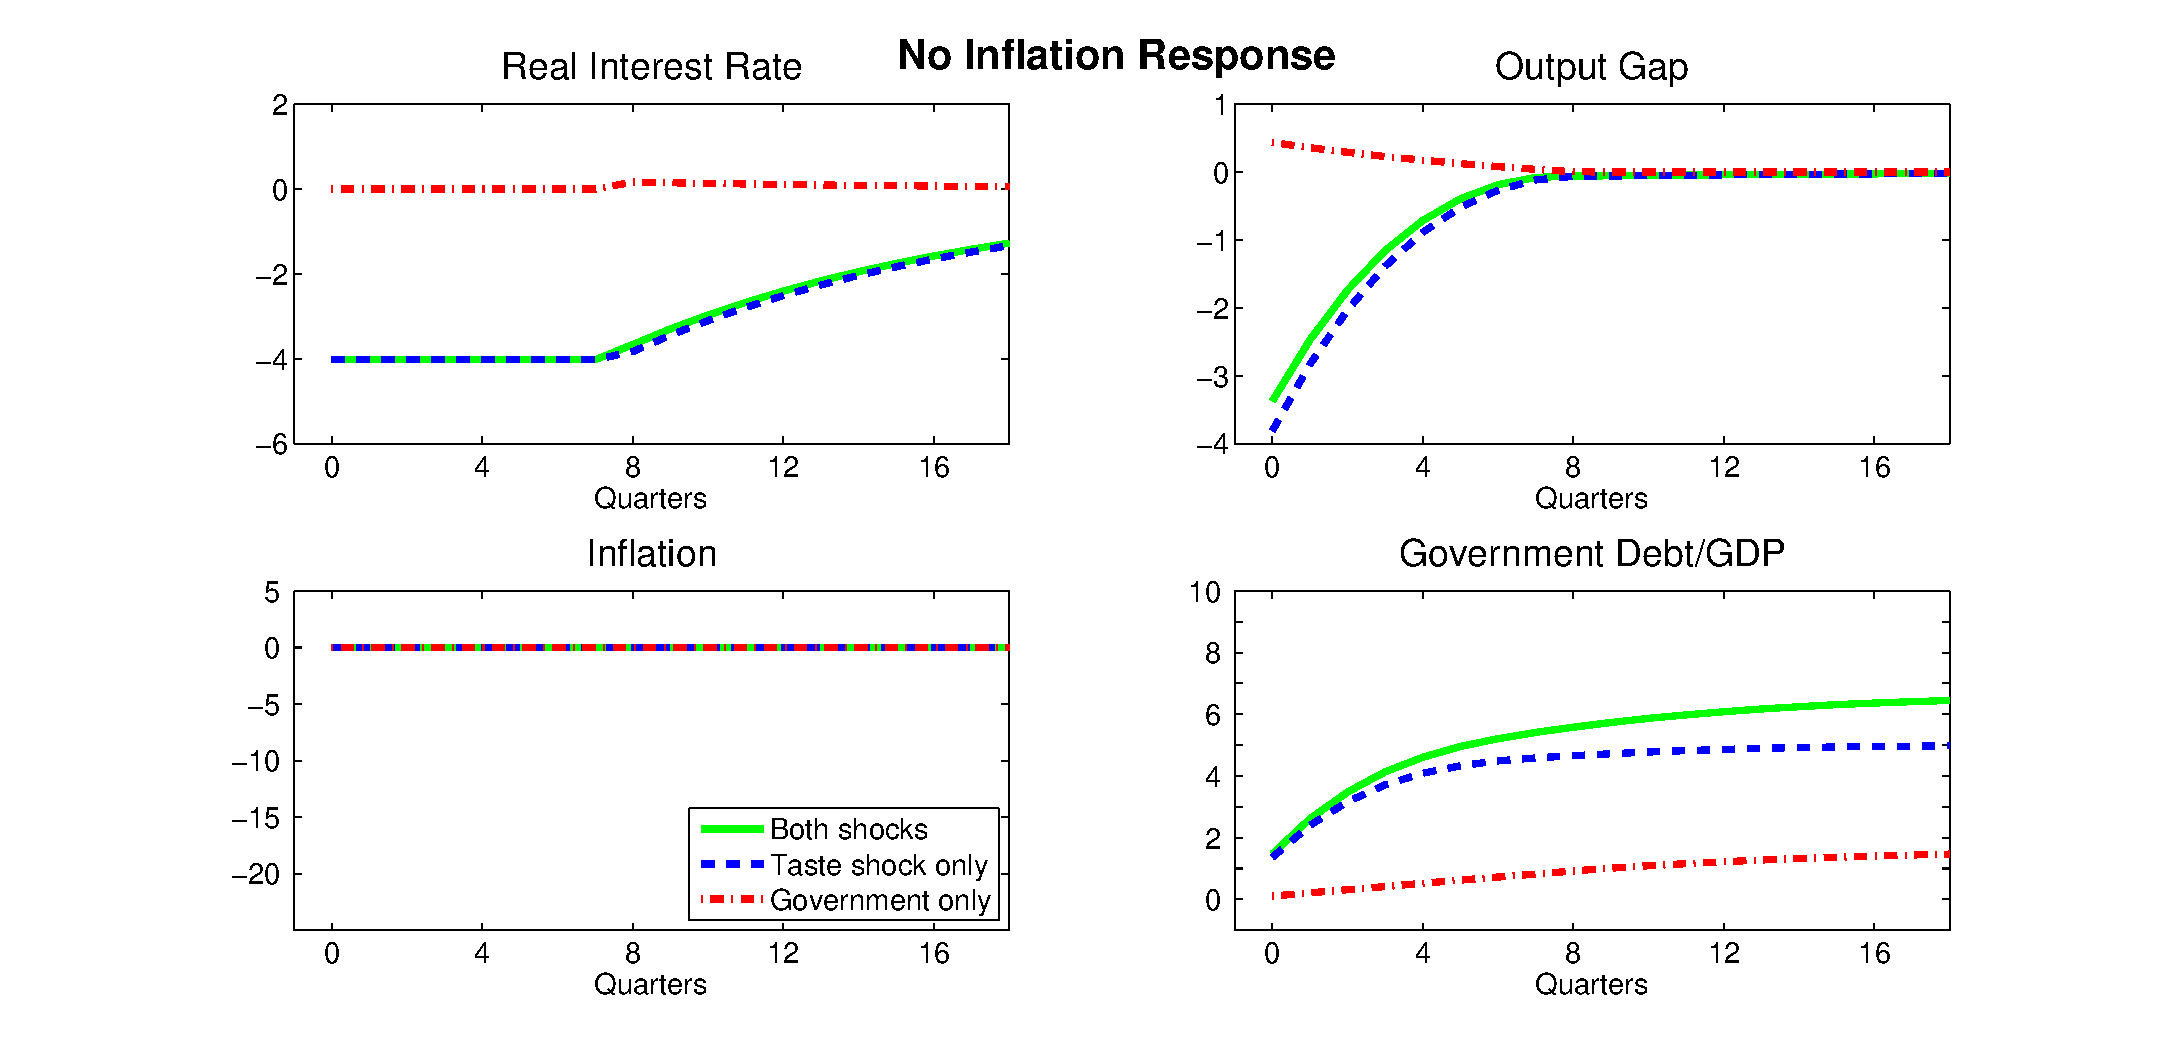
\includegraphics[width=\textwidth]{Paperpics/Figure2noIR}
\caption{Immediate Rise in Government Spending (No Inflation Response)}
\label{IRnoinflation}
\end{figure}
In the following subsections we explain the cruxes to get the right results. We explain more in detail the shock parameters, emphasize the role of the price rigidity and the policy responses to the negative taste shock.



\subsection*{The Shock Parameter}
The model consists of two different types of exogenous shocks: the consumption taste shock and the government spending shock. The adverse consumption shock triggers the fall of the potential real interest rate. We begin the analysis by setting the Calvo parameter equal to one and thus eliminating changes in inflation, to emphasize in the next sections the role of inflation in our model and on the government spending multiplier. For the following calculations and figures, it is important to find the exact values to get an eight quarter liquidity trap. The nominal and real interest rate fall simultaneously to the zero lower bound when the adverse consumption shock is large enough. The interest rates stay then at the lower bound for eight quarters and adjust continuously. The negative shock also leads to a fall in output and rise in government debt. In Figure \ref{IRnoinflation} to \ref{Figure1a} we calculate with a negative taste shock of $29.2$. The taste shock is scaled in the model by the scale parameter $\nu_c$ and $\left(1- g_y\right)$, which can be seen as the private sectors share of the steady-state output. Therefore, the negative taste shock can be interpreted as $0.01 * \left(1-0.2\right) * 29.2 = 0.2336$ or a $23,36\%$ fall in output of steady-state GDP.
\par
\bigskip
To counteract the negative effects on output, the government increases the spending by one percentage point of total GDP. The interpretation of the government spending shock is similar to the taste shock.  The government shock is scaled by the government share on total output $g_v$. We calculate in the model with a spending increase of $0.05$. This leads after scaling $0.2 * 0.05 = 0.01$ to the required government spending shock.
In Figure \ref{IRnoinflation} the solid green line shows the dynamic effects of both shocks, the blue dashed line the result of the negative taste shock without the rinse in spending and the red dash-dotted line the isolated effects of the government shock in the scenario of both shocks. It is important to mention that the red line is calculated by the difference between both shocks and the taste shock only to extract the effects of the government spending rise.
\par
\bigskip
Figure \ref{Figure1b} shows the consequences for the potential real interest rate when we loop the negative taste shock between $0$ and $50$ and then calculate the duration of the liquidity trap. The step function implies that a sightly larger adverse shock does not change the liquidity trap duration. Only when the potential real interest rate falls beyond a certain threshold, the adverse taste shock extends the liquidity trap duration. Figure \ref{Figure1bscatter} shows the scatter plot of the adverse taste shock. We loop the taste shock between the starting point $0$ and the end point $50$ with the increment of the sequence of $0.1$ and show the 501 shocks which enter the model to create the step function.
\begin{figure}[p]
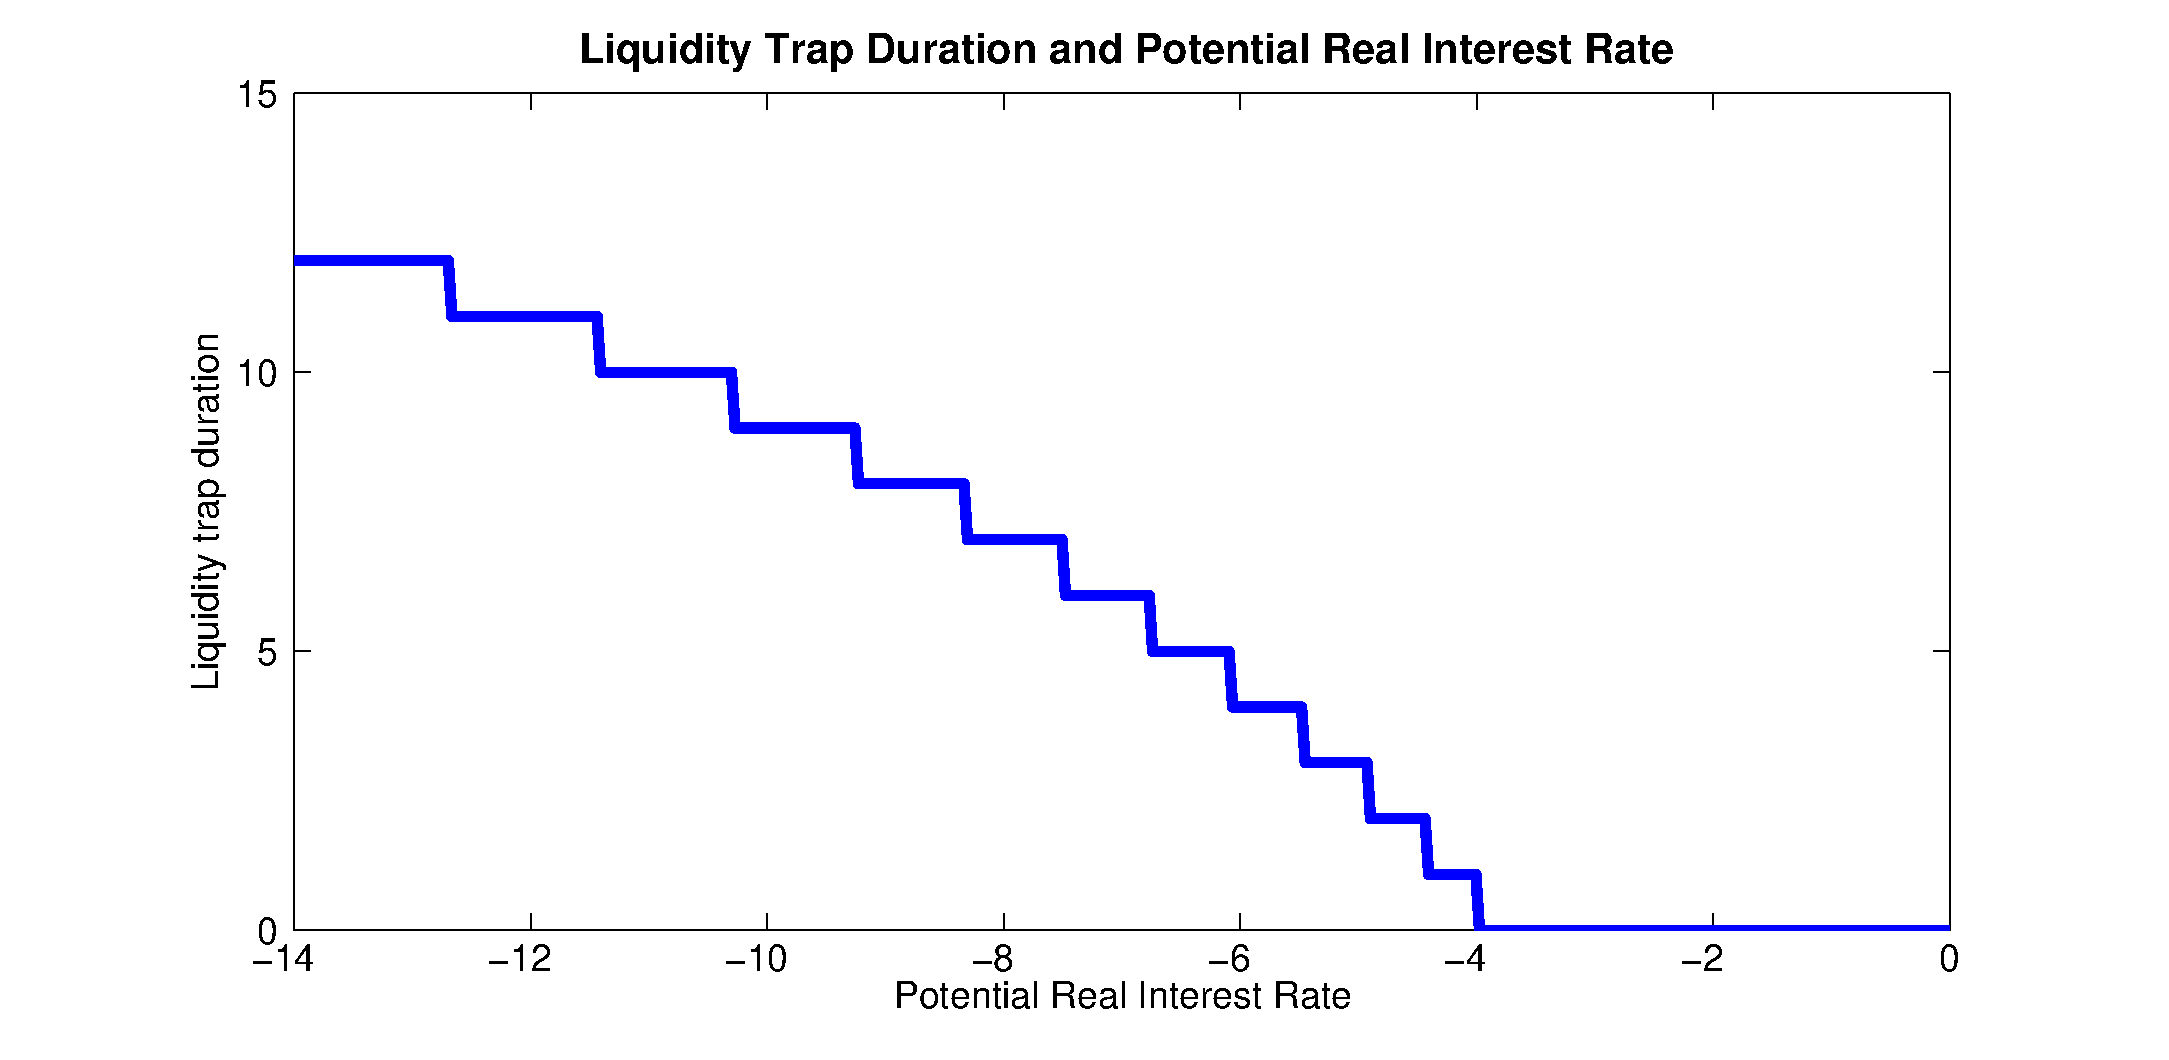
\includegraphics[width=\textwidth]{Paperpics/Figure1b}
\caption{Potential Real Interest Rate and Variation of Taste Shock}
\label{Figure1b}
\end{figure}

\begin{figure}[p]
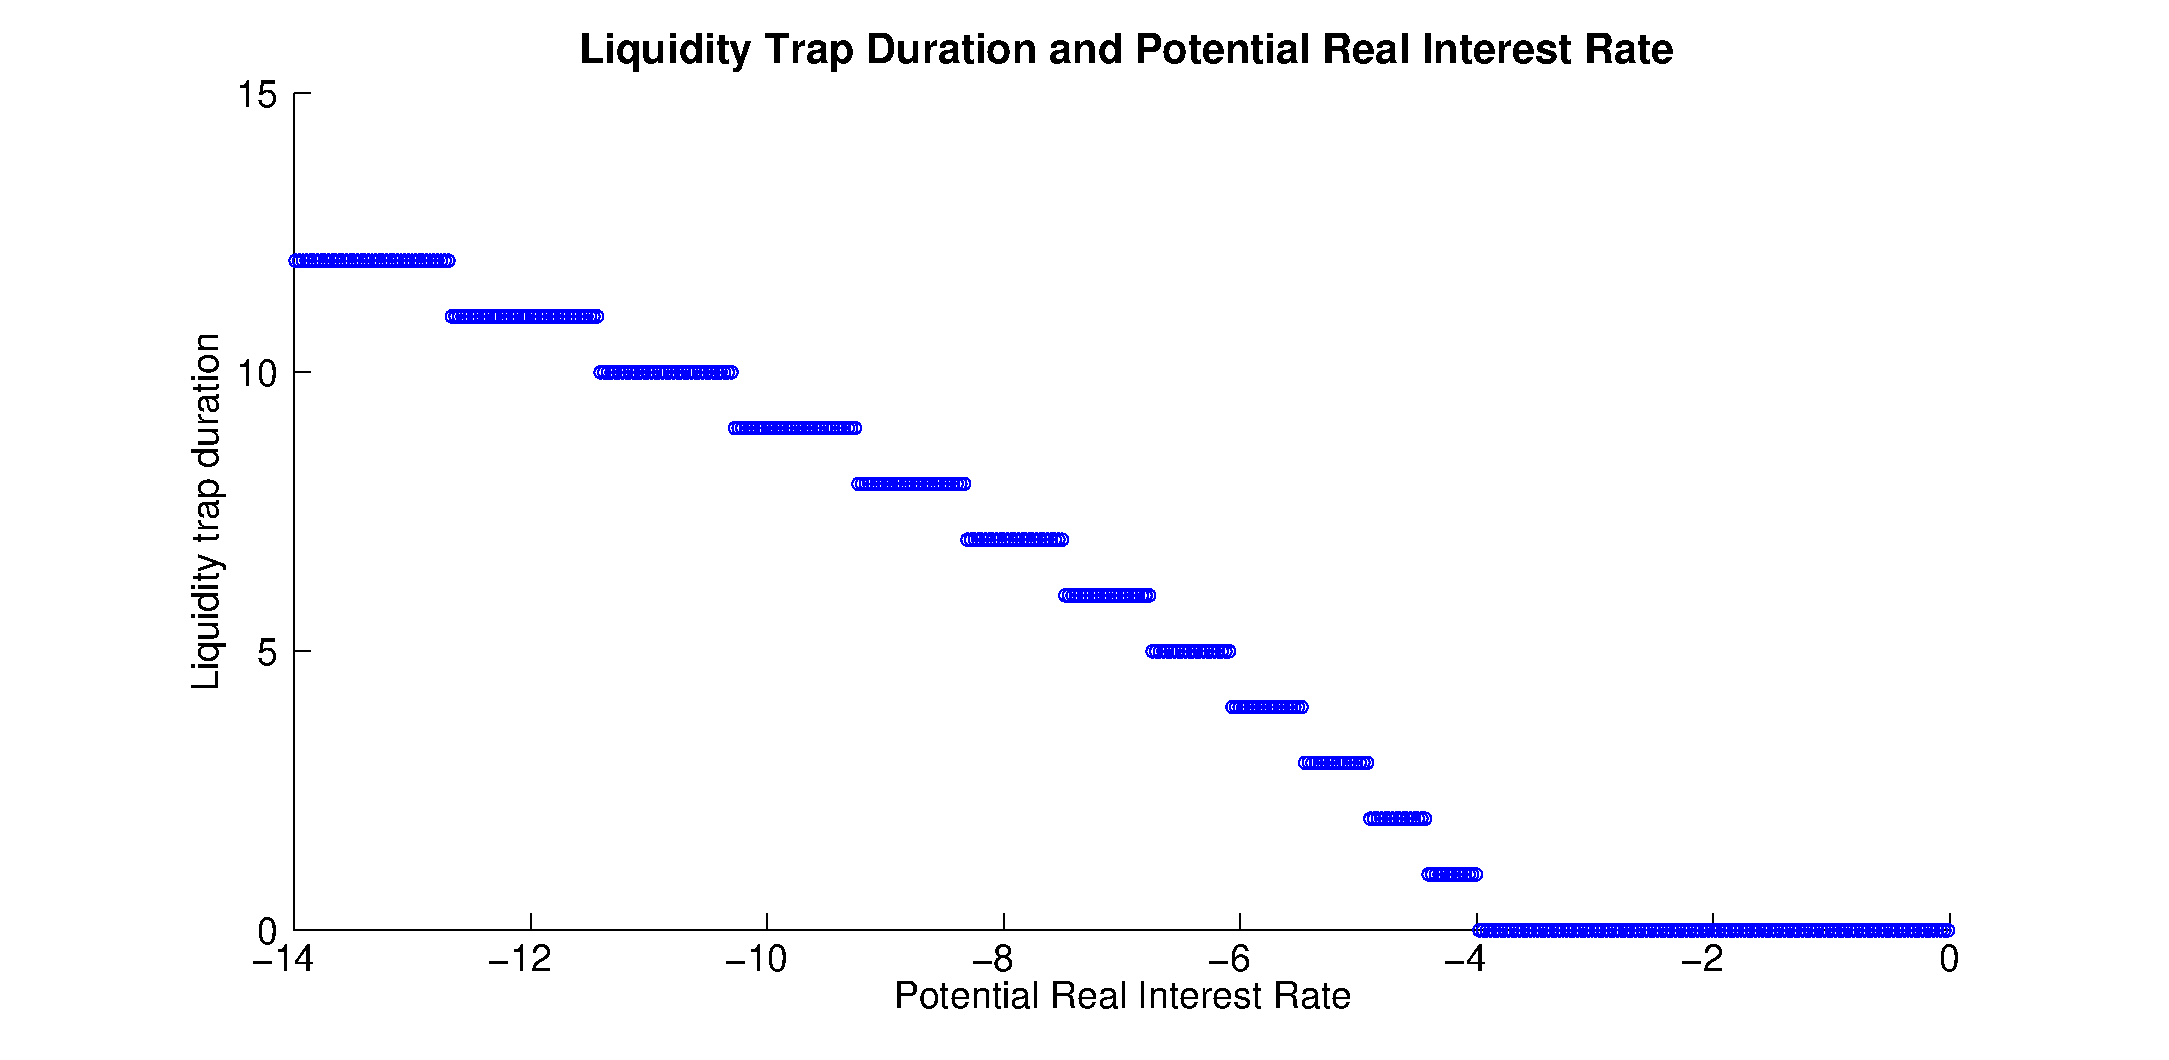
\includegraphics[width=\textwidth]{Paperpics/Figure1bscatter}
\caption{Potential Real Interest Rate and Variation of Taste Shock (Scatter plot)}
\label{Figure1bscatter}
\end{figure}





\subsection*{The Calvo Price Setting}
The slope of the Phillips curve is one important factor in the analysis of the government spending multiplier and the impact of fiscal spending on government debt. In Figure \ref{IRnoinflation}, we begin in an environment of zero inflation.
As the inflation is kept to zero, the annualized real interest rate falls to $-4\%$ and follows the path of the nominal interest rate $\left(r_t = i_t\right)$. We change the Calvo parameter to 0.8 to get a 5 quarter price contract duration in the model and thereby allow inflation to react. When the economy now hits the zero lower bound and inflation is responsive, the fall in output is very large. The exogenous shock leads to a fall in marginal costs and a decline in prices which changes the inflation expectations of the agents. Real interest rates have then to rise when the nominal interest rate is stuck at the zero lower bound. Consequently, households change their consumption behavior by increasing their savings which reduces the output even further.
\par
\bigskip
At the zero lower bound monetary policy cannot cut the nominal interest rate far enough. With falling inflation the real interest rate rises, triggering an even stronger fall in the output gap. When the nominal interest rate hits its lower bound, the central bank does not have any further options to react in our simple model. We see therefore that the real interest rate plays the key role at the ZLB in the NK model. In this framework fiscal policy becomes crucial to stabilizes the economy and counteract the negative taste shock. Figure \ref{IR5quarter} supports strongly economic theory and this results.

\begin{figure}[p]
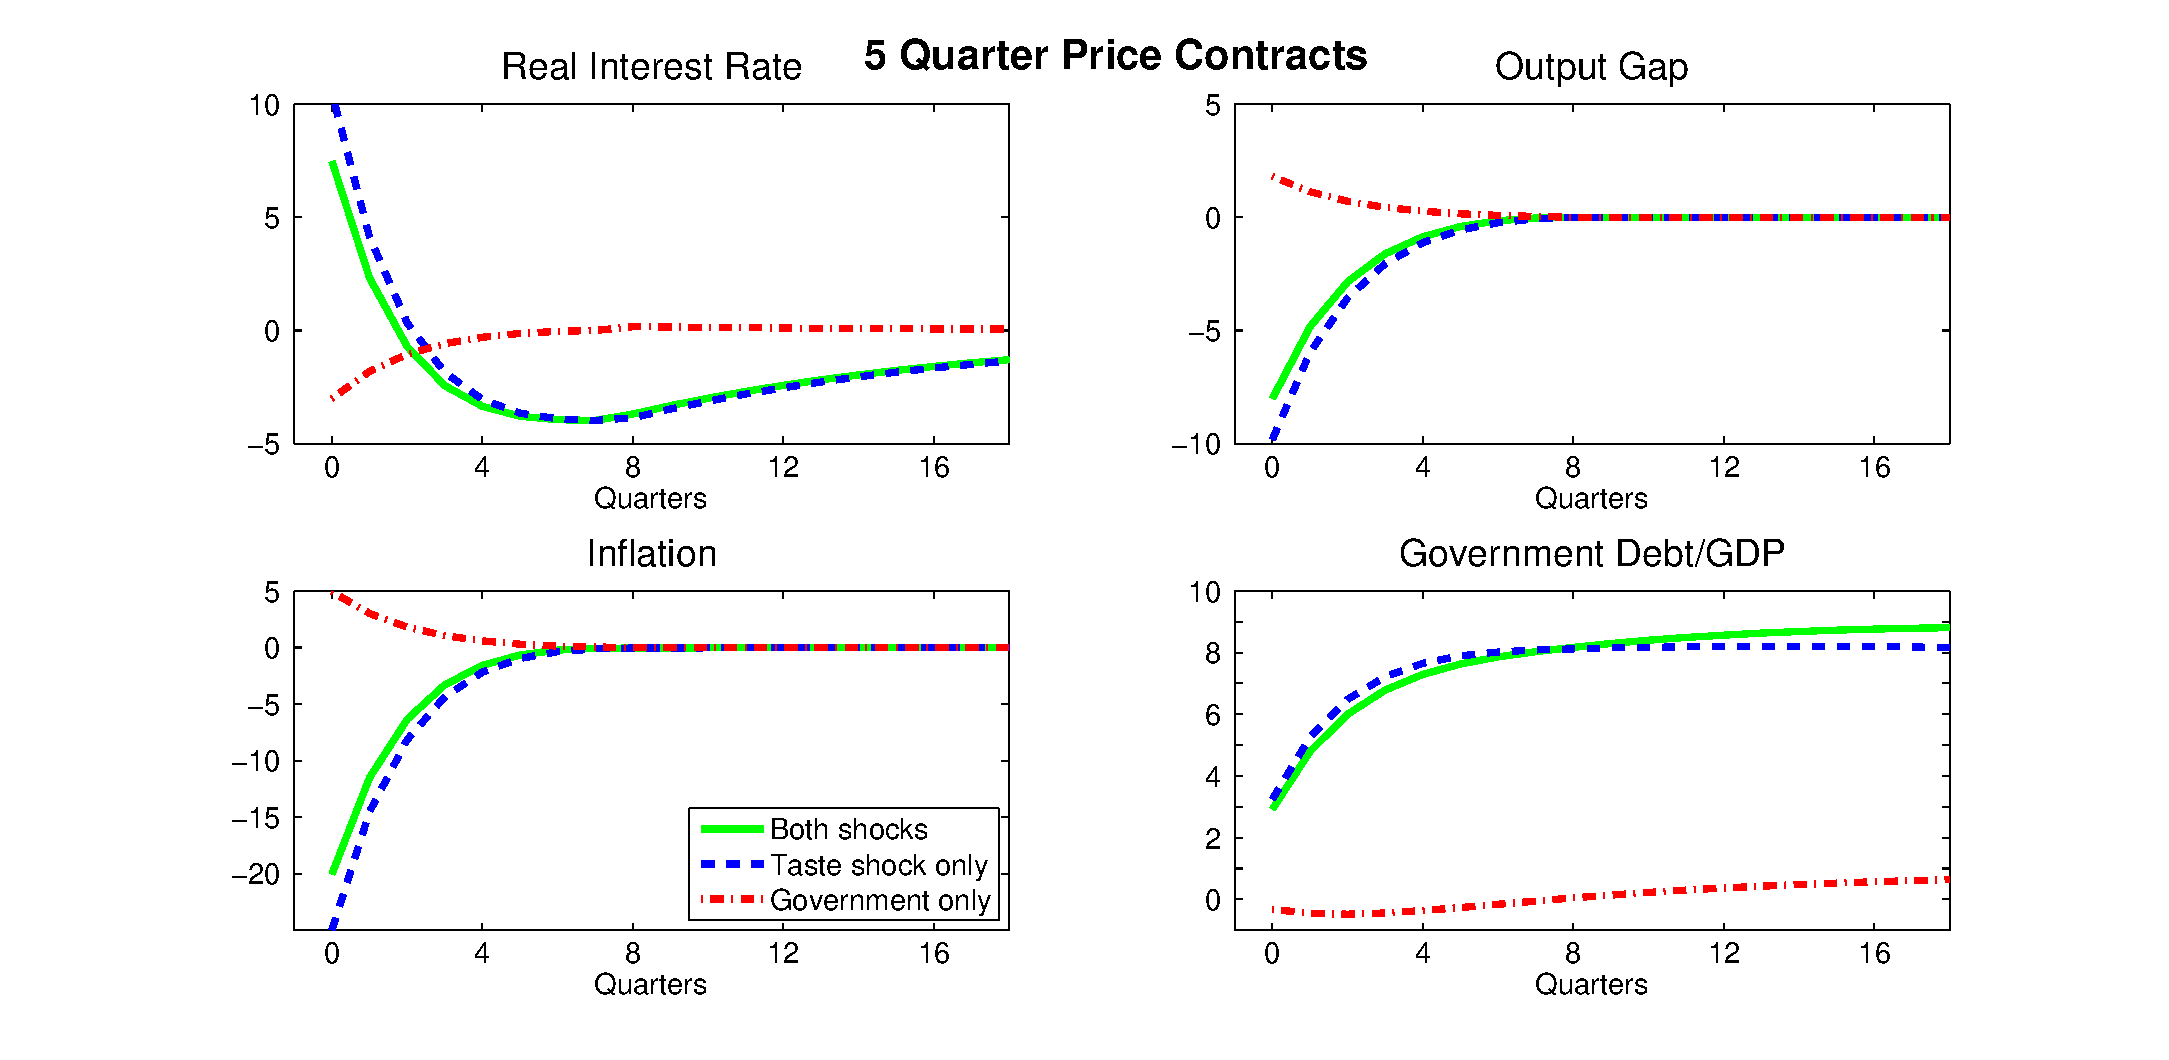
\includegraphics[width=\textwidth]{Paperpics/Figure25quarter}
\caption{Immediate Rise in Government Spending (5 Quarter Price Contracts)}
\label{IR5quarter}
\end{figure}


\subsection*{Policy rules}
In the following, we shift the focus to the monetary and fiscal policy rules. After setting the parameters of the monetary rule in Figure \ref{IR5quarter} arbitrarily large, we change the monetary policy rule to values which are more \textit{usual} in standard New Keynesian models. We set the Taylor rule parameter on output $\gamma_x$ to 0.2 and inflation $\gamma_{\pi}$ to 1.5. As a result the negative taste shock leads to an explosion in the impulse response. The amplitude reaches to limits which can be seen as quite unrealistic and not useful for further economic analysis. The careful calibration of the Taylor rule parameter must be seen as essential in our model and part of of an optimal monetary policy analysis.
\par
\bigskip
We turn the focus now on the fiscal response to the negative taste shock. Figure \ref{Figure1a} shows how the rise in government spending helps to shorten the liquidity trap duration. The negative taste shock leads to a fall in the potential real interest rate and keeps $r^{pot}$ below the nominal interest rate for eight quarters. Fiscal policy partly offsets this drop and pushes the potential real interest rate upwards. Nevertheless, the spending increase of $1\%$ of total GDP is still not high enough to shorten the liquidity trap duration. Not till the fiscal response exceeds a certain threshold, the liquidity trap duration changes to seven quarters or even lower. The $2\%$ spending hike yet reduces the duration of the liquidity trap and the central bank can raise the nominal interest rate after seven quarters.
Figure \ref{Figure1a} gives a first important insight into the analysis of the marginal and average government spending multiplier, we undertake in the following sections.

\begin{figure}[p]
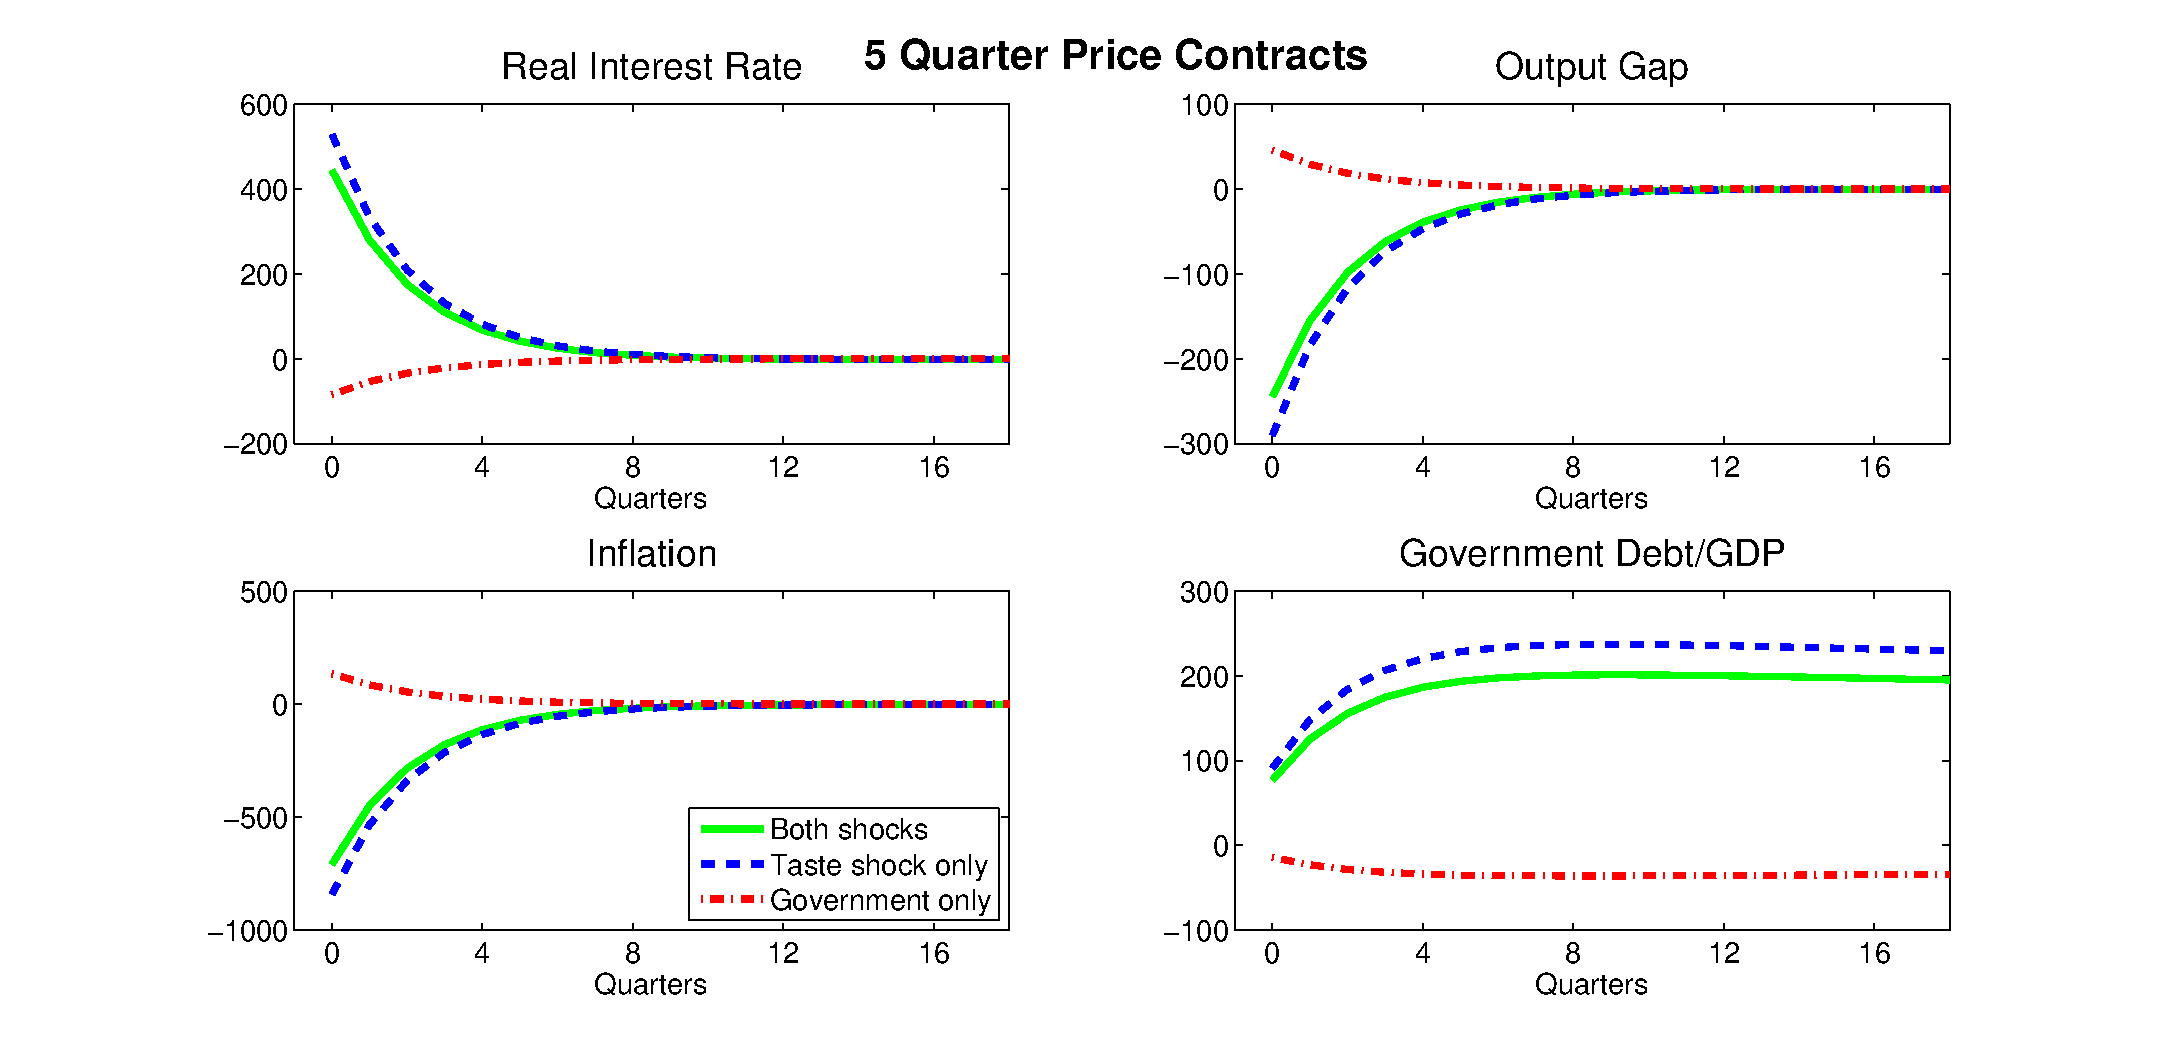
\includegraphics[width=\textwidth]{Paperpics/Figure25quarternewtaylorrule}
\caption{Immediate Rise in Government Spending (Alternative Taylor Rule Values)}
\label{IR5quarternewtr}
\end{figure}
\bigskip

\begin{figure}[p]
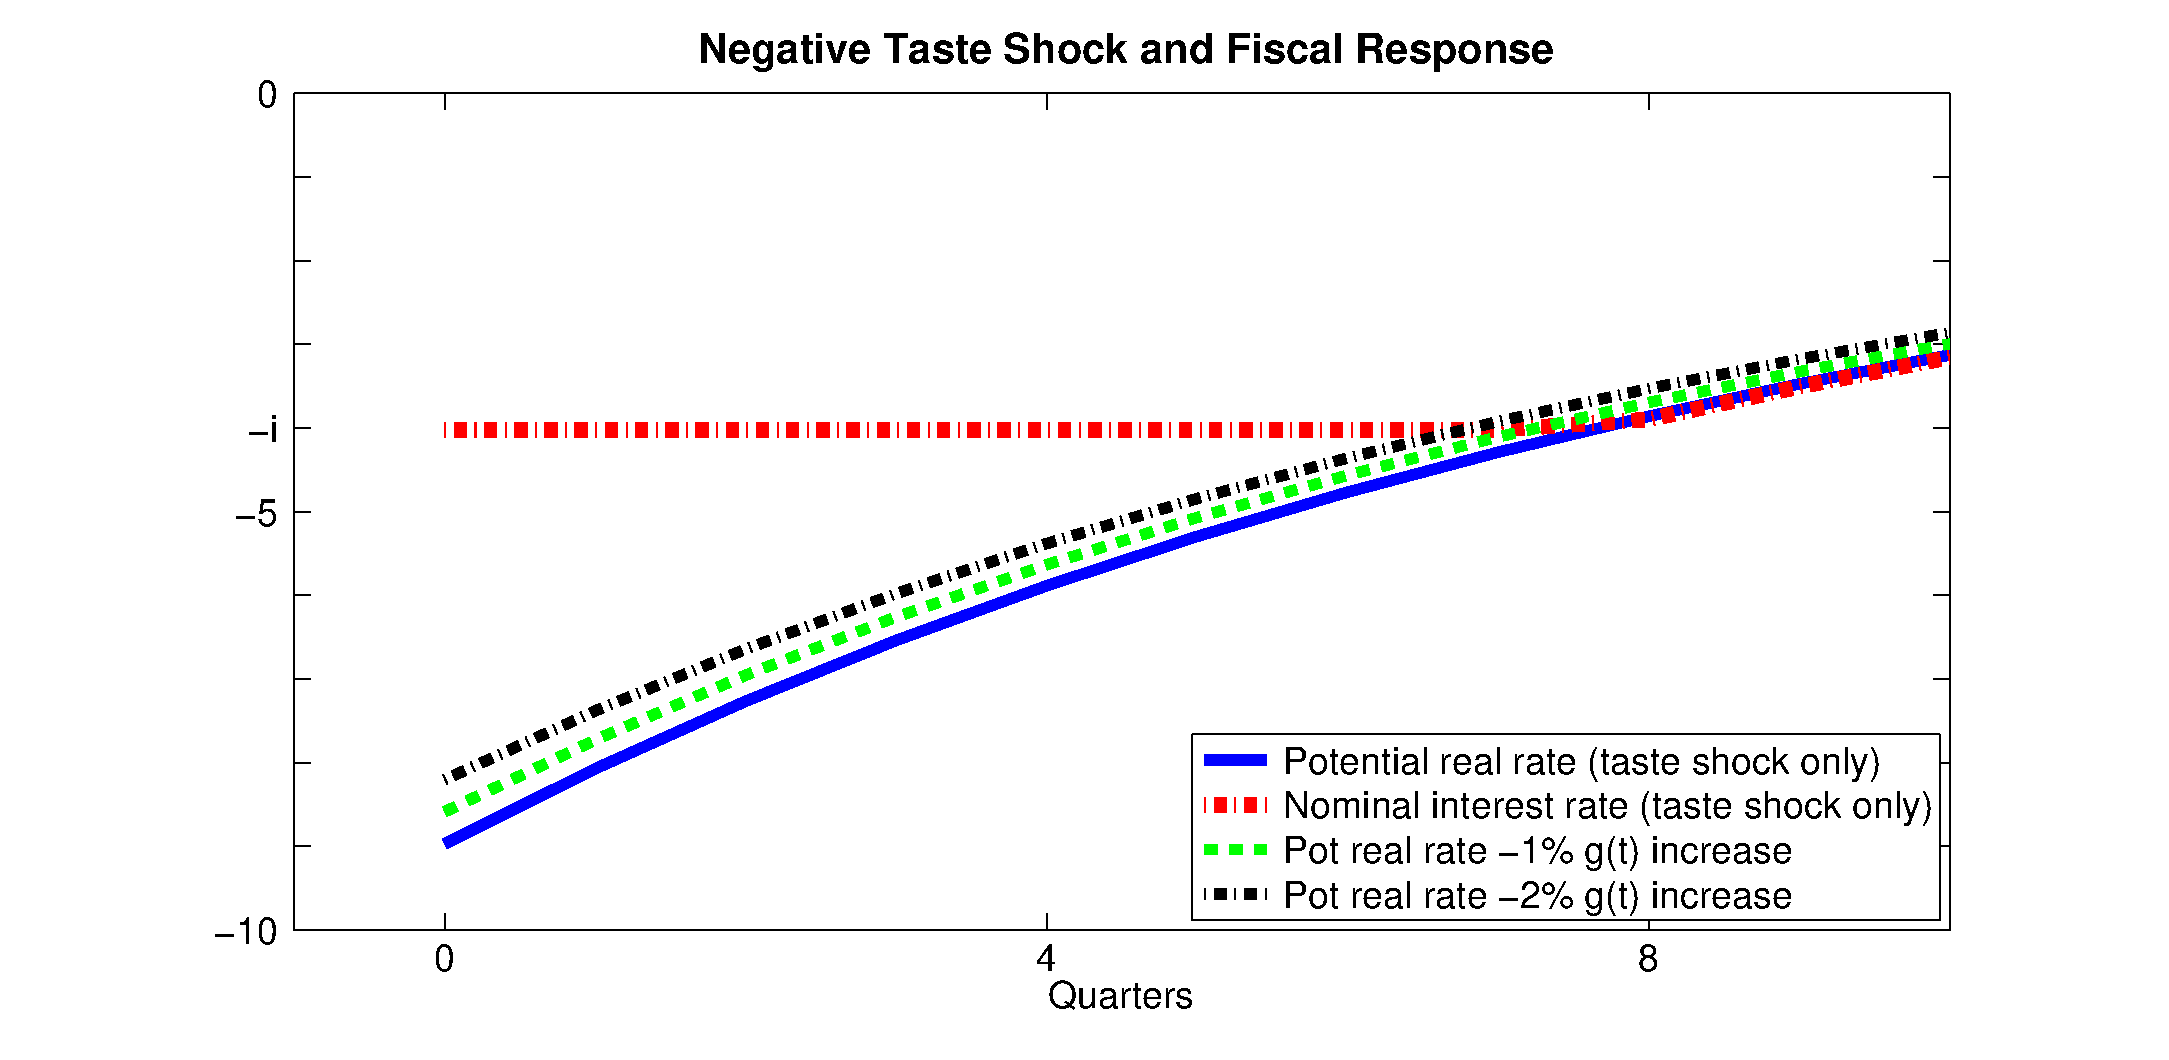
\includegraphics[width=\textwidth]{Paperpics/Figure1a}
\caption{Potential Real Interest Rate and Fiscal Response}
\label{Figure1a}
\end{figure}



\input{Multiplier}
\section{Workflow}

\subsection*{GitHub}
\label{sub:GitHub}

To coordinate and control our coding, we have used GitHub\footnote{https://github.com}. GitHub is version control software based on the git system. It allows its users to keep track of all the changes made to a specific project and provides an overview of the its development. GitHub has a variety of features and it is mostly used by software engineers who work simultaneously with many other people in big projects. GitHub was particularly useful to us because it forced us to document all the changes we made to the project. This way it was much easier for us two to work remotely without losing track of what each other had already done.

Alongside with the documentation function, the git system offers the possibility to reload previous versions of the project and undo changes that turn out to be undesired. GitHub displays a timeline in which the user can follow the development of the project from its beginning until its current state. This allows the user to go back in time and recover old versions of project or only parts of it. This was particularly useful for us too. It happened more than once that one of us two has mistakenly changed the code and Dynare could no longer simulate the model. Instead of spending hours debugging and trying to find the error, we simply opted to go back to a previous version and start again from there.

Although the git system is primarily designed to be used from the command line (Terminal for macOS or Command Line for Windows), GitHub offers a very user-friendly desktop application, which makes possible for not-so-advanced user to profit from its features. GitHub is free as long as you are willing to make your project public. The code for this project, for example, is available online \footnote{https://github.com/denismaciel/fiscalfreelunch}.


\subsection*{Syntax Highlighting}
\label{sub:Syntax Highlighting}

Another tip worth mentioning is to use syntax highlighting while coding. It is not only much more comfortable to read a code whose parts have different colors according to its function, but the task of spotting errors becomes much easier when the code is highlighted. Even though we could not find a specific syntax highlighting package for Dynare, it turns out that Java's highlighting works well with Dynare. For example, \% is used to comment the code and that single feature makes worth trying it.


%Include footnote with link to our github project
%maybe include screenshot of github


\section{Conclusion}

 




\pagebreak[4]
\addcontentsline{toc}{section}{References}
\bibliographystyle{plainnat}  %Zitationsstil
\bibliography{References}


%Grafiken

% \begin{figure}[th]
% \includegraphics[width=\textwidth]{Paperpics/}
% \caption{Spending Multiplier in a simple New Keynesian Model (No Inflation Response)}
% \label{GSMnoinflation}
% \end{figure}
% \bigskip
%
% \begin{figure}[th]
% \includegraphics[width=\textwidth]{Paperpics/}
% \caption{Multiplier Schedule: Implications to Y and G}
% \label{MultiplierSchedule}
% \end{figure}
% \bigskip
%
% \begin{figure}[th]
% \includegraphics[width=\textwidth]{Paperpics/}
% \caption{Spending Multiplier in a simple New Keynesian Model (Alternative Price Contract Duration)}
% \label{GSMalternativeprices}
% \end{figure}
% \bigskip
%
% \begin{figure}[th]
% \includegraphics[width=\textwidth]{Paperpics/}
% \caption{Government Debt Response in a simple New Keynesian Model (No Inflation Response)}
% \label{GovernmentDebtnoinflation}
% \end{figure}
% \bigskip
%
% \begin{figure}[th]
% \includegraphics[width=\textwidth]{Paperpics/}
% \caption{Government Debt Response in a simple New Keynesian Model (Alternative Price Contract Duration}
% \label{GovernmentDebtalternativeprices}
% \end{figure}
% \bigskip



%Tabellen
\newpage

\begin{table}[th]
\centering
\caption{Parameter Values Benchmark Calibration}
\bigskip
\bgroup
\def\arraystretch{1.5}
\begin{tabular}{p{1.2cm} l c}
\toprule\toprule \noalign{\smallskip}
 & \multicolumn{1}{c}{\textit{Description}} & \textit{Value} \\
\hline\noalign{\smallskip}

$\alpha$ & Capital Share   & 0.3 \\
$\beta$  & Discount Factor & 0.995 \\
$\sigma$ & Intertemporal Substitution Elasticity & 1 \\
$\chi$ & Inverse of Frisch-Elasticity & 2.5 \\
$g_y$ & Government Share on Output & 0.2 \\
$\varphi_b$ & Tax Rule Parameter & 0.01 \\
$\nu_c$ & Scale Parameter on the Taste Shock & 0.01 \\
$\rho$ & AR(1) Natural Rate for both Shocks & 0.1 \\
$\xi_p$ & Calvo Parameter (No Inflation) & 1 \\
 & Calvo Parameter (10 quarter price contracts) & 0.9 \\
 & Calvo Parameter (5  quarter price contracts) & 0.8 \\
 & Calvo Parameter (4  quarter price contracts) & 0.75 \\
 & Calvo Parameter (3  quarter price contracts) & 0.667 \\
$\gamma_{\pi}$ & Taylor Rule Coefficient on Inflation & 66.15 \\
$\gamma_x$ & Taylor Rule Coefficient on Output Gap & 66.15 \\
\bottomrule
\end{tabular}
\egroup
\label{tab:Tabel1}
\end{table}


\end{document}
